\documentclass[11pt]{beamer}
\usetheme{CambridgeUS}
\usepackage[utf8]{inputenc}
\usepackage{amsmath}
\usepackage{amsfonts}
\usepackage{amssymb}
\author{Volgushev et al.}
\title{Distributed Inference for Quantile Regression Process}
%\setbeamercovered{transparent} 
%\setbeamertemplate{navigation symbols}{} 
%\logo{} 
%\institute{} 
%\date{} 
%\subject{} 
\begin{document}
\newcommand{\cX}{\mathcal{X}}
\begin{frame}
\titlepage
\end{frame}

%\begin{frame}
%\tableofcontents
%\end{frame}

\section{Introduction}
\begin{frame}{Quantile Regression}
Given data $\{X_i,Y_i\}$,quantile regression for such models is classically
formulated through the following minimization problem:
\begin{equation}\tag{1.1}
\widehat{\boldsymbol{\beta}}_{o r}(\tau):=\arg \min _{\mathbf{b} \in \mathbb{R}^{m}} \sum_{i=1}^{N} \rho_{\tau}\left\{Y_{i}-\mathbf{b}^{\top} \mathbf{Z}\left(X_{i}\right)\right\},
\end{equation}
where $\rho_{\tau}(u):=:=\{\tau-\mathbf{1}(u \leq 0)\} u$.


\end{frame}

\begin{frame}{Divide and Conquer}
\begin{itemize}
\item $N=Sn$: N observations, $S$ machines with $n$ observations each.
\item Apply statistical procedures on each machine(worker) and transmit the result to the centre machine(master).
\end{itemize}
\end{frame}

\begin{frame}{Notation}
\begin{itemize}
\item Let $\mathcal{X}:=supp(X)$.
\item Let $Z=Z(X)$ and $Z_i=Z(X_i)$ and assume $\mathcal{T}=\left[\tau_{L}, \tau_{U}\right]$ for some $0<\tau_L<\tau_U<1$.
\item $\mathcal{S}^{m-1} \subset \mathbb{R}^{m}$ is the unit sphere.
\item $a_{n} \asymp b_{n}$ means that $\left(\left|a_{n} / b_{n}\right|\right)_{n \in \mathbb{N}}$ and $\left(\left|b_{n} / a_{n}\right|\right)_{n \in \mathbb{N}}$ are bounded.
\item Define the class of functions
$$
\begin{array}{c}
\Lambda_{c}^{\eta}(\mathcal{T}):=\left\{f \in \mathcal{C}^{\lfloor\eta\rfloor}(\mathcal{T}): \sup _{j \leq\lfloor\eta\rfloor } \sup_{\tau \in \mathcal{T}} \left|D^{j} f(\tau)\right| \leq c\right. \\
\left.\sup _{j=\lfloor\eta \rfloor}\sup_{ \tau \neq \tau^{\prime}} \frac{\left|D^{j} f(\tau)-D^{j} f\left(\tau^{\prime}\right)\right|}{\left\|\tau-\tau^{\prime}\right\|^{\eta-\lfloor\eta\rfloor}} \leq c\right\},
\end{array}
$$
where $\eta$ is called the "degree of H\"older continuity", and $\mathcal{C}^{\alpha}(\mathcal{X})$ denotes the
class of $\alpha$-continuously differentiable functions on a set $\mathcal{X}$.
\end{itemize}
\end{frame}

\section{A two step Procedure}
\begin{frame}{The model}
We consider a general approximately linear model:
$$
Q(x;\tau)\approx Z(x)^{T}\beta_{N}(\tau).
$$
In this paper, we focus on three classes of transformation $Z(x)\in \mathbb{R}^m$ which include many models as special cases:
\begin{itemize}
\item fixed and finite $m$
\item diverging $m$ with local support structure(B-splines)
\item diverging $m$ without local support structure
\end{itemize}
\end{frame}
\begin{frame}{The divide and conquer algorithm}
\begin{itemize}
\item Divide the data $\{(X_i,Y_i)\}_{i=1}^N$ into $S$ sub-samples of size $n$. Denote the $s$-th sub-sample as $\left\{\left(X_{i s}, Y_{i s}\right)\right\}_{i=1}^{n}$ where $s=1,2,\dots,S$.
\item For each $s$ and $\tau$, estimate the sub-sample based quantile regression coefficient as follows:
$$
\widehat{\boldsymbol{\beta}}^{s}(\tau):=\arg \min _{\boldsymbol{\beta} \in \mathbb{R}^{m}} \sum_{i=1}^{n} \rho_{\tau}\left\{Y_{i s}-\boldsymbol{\beta}^{\top} \mathbf{Z}\left(X_{i s}\right)\right\}.
$$
\item  Each local machine sends $\widehat{\boldsymbol{\beta}}^{s}(\tau) \in \mathbb{R}^{m}$ to the master that outputs a
pooled estimator
$$
\overline{\boldsymbol{\beta}}(\tau):=S^{-1} \sum_{s=1}^{S} \widehat{\boldsymbol{\beta}}^{s}(\tau).
$$
\end{itemize}
\end{frame}

\begin{frame}{Quantile Projection}
\begin{itemize}
\item While $\bar{\beta}(\tau)$ gives an estimator at a fixed $\tau\in \mathcal{T}$, a complete picture of the conditional distribution is often desirable.
\item To achieve this, we
propose a two-step procedure. First compute  $\overline{\boldsymbol{\beta}}\left(\tau_{k}\right) \in \mathbb{R}^{m}$ for each $\tau_{k} \in \mathcal{T}_{K}$, where $\mathcal{T}_{K} \subset \mathcal{T}=\left[\tau_{L}, \tau_{U}\right]$ is grid of quantile values in $\mathcal{T}$ with $|\mathcal{T}_K|=K\in \mathbb{N}$.
\item Second project each component of the vectors $\left\{\overline{\boldsymbol{\beta}}\left(\tau_{1}\right), \ldots, \overline{\boldsymbol{\beta}}\left(\tau_{K}\right)\right\}$  on a space
of spline functions in $\tau$. 
\end{itemize}
\end{frame}

\begin{frame}{Quantile Projection}
Let
$$
\widehat{\boldsymbol{\alpha}}_{j}:=\arg \min _{\boldsymbol{\alpha} \in \mathbb{R}^{q}} \sum_{k=1}^{K}\left(\bar{\beta}_{j}\left(\tau_{k}\right)-\boldsymbol{\alpha}^{\top} \mathbf{B}\left(\tau_{k}\right)\right)^{2}, \quad j=1, \ldots, m,
$$
where $ \mathbf{B}:=(B_1,\dots,B_q)^T$ is a B-spline basis defined on G equidistant knots $\tau_{L}=t_{1}<\ldots<t_{G}=\tau_{U}$ with degree $r_{\tau}\in \mathbb{N}$. Using $\widehat{\boldsymbol{\alpha}}_{j}$, we define 
$$
\widehat{\boldsymbol{\beta}}(\tau):=\widehat{\Xi}^{\top} \mathbf{B}(\tau),
$$
where
$$
\widehat{\Xi}:=\left[\widehat{\boldsymbol{\alpha}}_{1} \widehat{\boldsymbol{\alpha}}_{2} \ldots \widehat{\boldsymbol{\alpha}}_{m}\right].
$$
{\color{blue}
The $j$th element $\widehat{\beta}_{j}(\tau)=\widehat{\alpha}_{j}^{\top} \mathbf{B}(\tau)$ can be viewed as projection,with respect to $||f||_K:=(\sum_{k=1}^K f^2(\tau_k))^{1/2}$ of $\bar{
\beta}_j$ onto the
polynomial spline space with basis $B_1,\dots,B_q$. In what follows, this projection
is denoted by $\Pi_k$.}
\end{frame}

\begin{frame}{Quantile Projection}
The algorithm for computing the quantile projection matrix $\widehat{\Xi}$ is summarized below, here the divide-and-conquer is applied as a subroutine:
\begin{itemize}
\item Define a 	grid of quantile levels $\tau_{k}=\tau_{L}+(k / K)\left(\tau_{U}-\tau_{L}\right)$ for $k=1,\dots,K$. For each $\tau_k$, compute $\bar{\beta}(\tau_k)$.
\item For each $j=1,\dots,m$, compute
$$
\widehat{\boldsymbol{\alpha}}_{j}=\left(\sum_{k=1}^{K} \mathbf{B}\left(\tau_{k}\right) \mathbf{B}\left(\tau_{k}\right)^{\top}\right)^{-1}\left(\sum_{k=1}^{K} \mathbf{B}\left(\tau_{k}\right) \bar{\beta}_{j}\left(\tau_{k}\right)\right),
$$
which is a closed form solution.
\item Set the matrix
$$
\hat{\Xi}:=\left[\widehat{\boldsymbol{\alpha}}_{1} \widehat{\boldsymbol{\alpha}}_{2} \ldots \widehat{\boldsymbol{\alpha}}_{m}\right].
$$
\end{itemize}
\end{frame}

\begin{frame}{Conditional distribution}
A direct application of the above algorithm is to estimate the quantile function for any $\tau \in \mathcal{T}$.
More precisely, we consider
$$
\widehat{F}_{Y | X}(y | x):=\tau_{L}+\int_{\tau_{L}}^{\tau_{U}} 1\left\{\mathbf{Z}(x)^{\top} \widehat{\boldsymbol{\beta}}(\tau)<y\right\} d \tau,
$$
where $\tau_L$ and $\tau_U$ are chosen close to 0 and  1.
The intuition behind this
approach is the observation that
$$
\tau_{L}+\int_{\tau_{L}}^{\tau_{U}} 1\{Q(x ; \tau)<y\} d \tau=\left\{\begin{array}{ll}
\tau_{L} & \text { if } F_{Y | X}(y | x)<\tau_{L} \\
F_{Y | X}(y | x) & \text { if } \tau_{L} \leq F_{Y | X}(y | x) \leq \tau_{U} \\
\tau_{U} & \text { if } F_{Y | X}(y | x)>\tau_{U}
\end{array}\right.
$$
The function $\hat{F}_{Y|X}$ is smooth functional of the map $\tau \mapsto \mathbf{Z}(x)^{\top} \widehat{\boldsymbol{\beta}}(\tau)$.
\end{frame}

\section{Theoretical analysis}
\begin{frame}{Conditions}
The following regularity conditions are needed
throughout this paper.
\begin{itemize}
\item[(A1)] {\color{blue} Assume that $\left\|\mathbf{Z}_{i}\right\| \leq \xi_{m}<\infty$ where $\xi_m$ is allowed to diverge}, and that
$1 / M \leq \lambda_{\min }\left(\mathbb{E}\left[\mathbf{Z Z}^{\top}\right]\right) \leq \lambda_{\max }\left(\mathbb{E}\left[\mathbf{Z Z}^{\top}\right]\right) \leq M$ holds uniformly in $N$ for some fixed constant $M$.
\item[(A2)]  The conditional distribution $F_{Y|X}(y|x)$  is twice differentiable w.r.t. y, with the corresponding derivatives $f_{Y | X}(y | x)$ and $f^{'}_{Y | X}(y | x)$.Assume
$\bar{f}:=\sup _{y \in \mathbb{R}, x \in \mathcal{X}}\left|f_{Y | X}(y | x)\right|<\infty, \overline{f^{\prime}}:=\sup _{y \in \mathbb{R}, x \in \mathcal{X}}\left|f_{Y | X}^{\prime}(y | x)\right|<\infty$ uniformly in $N$.
\item[(A3)] Assume that uniformly in N, there exists a constant $f_{\min}<\bar{f}$ such that
$$
0<f_{\min } \leq \inf _{\tau \in \mathcal{T}} \inf _{x \in \mathcal{X}} f_{Y | X}(Q(x ; \tau) | x).
$$
\end{itemize}
In these assumptions, we explicitly work with triangular array asymptotics for  $\{(X_i,Y_i)\}_{i=1}^N$, where $d=dim(X_i)$ is allowed to grow as well.
\end{frame}


\begin{frame}{Fixed dimensional linear models.}
In this section, we assume for all $\tau\in \mathcal{T}$ and $x \in \mathcal{X}$,
$$
Q(x ; \tau)=\mathbf{Z}(x)^{\top} \boldsymbol{\beta}(\tau),
$$
where $Z(X)$ has fixed dimension m. This simple model setup allows us to
derive a simple and clean bound on the difference between $\bar{\beta},\hat{\beta}$ and the oracle estimator $\hat{\beta}_{or}$ .
\end{frame}
\begin{frame}{Theorem 3.1}
Assume conditions (A1)-(A3) hold and that $K \ll N^2, S=o(N(\log N)^{-1})$. Then
$$
\sup _{\tau \in \mathcal{T}_{K}}\left\|\overline{\boldsymbol{\beta}}(\tau)-\widehat{\boldsymbol{\beta}}_{o r}(\tau)\right\|=O_{P}\left(\frac{S \log N}{N}+\frac{S^{1 / 4}(\log N)^{7 / 4}}{N^{3 / 4}}\right)+o_{P}\left(N^{-1 / 2}\right)
$$
If additionally $
K \gg G \gg 1$ we also have
$$
\begin{aligned}
\sup _{\tau \in \mathcal{T}}\left|\mathbf{Z}\left(x_{0}\right)^{\top}\left(\widehat{\boldsymbol{\beta}}(\tau)-\widehat{\boldsymbol{\beta}}_{o r}(\tau)\right)\right| \leq & O_{P}\left(\frac{S \log N}{N}+\frac{S^{1 / 2}(\log N)^{2}}{N}\right) \\
&+o_{P}\left(N^{-1 / 2}\right)\\
&+\sup _{\tau \in \mathcal{T}}\left|\left(\Pi_{K} Q\left(x_{0} ; \cdot\right)\right)(\tau)-Q\left(x_{0} ; \tau\right)\right|
\end{aligned}.
$$
\end{frame}


\begin{frame}{Notation}
Denote by $\mathcal{P}_{1}\left(\xi_{m}, M, \bar{f}, \overline{f^{\prime}}, f_{\min }\right)$ all pairs $(P,Z)$ of distributions P and transformations Z satisfying (3.1) and (A1)-(A3) with constants $0<\xi_{m}, M, \bar{f}, \overline{f^{\prime}}<\infty, f_{\min }>0$.
Since $m, \xi_m$ are constant in this
section, we use the shortened notation $\mathcal{P}_{1}\left(\xi, M, \bar{f}, \overline{f^{\prime}}, f_{\min }\right)$
\end{frame}

\begin{frame}{Oracle Estimator }
Under (A1)-(A3) it was developed in Belloni et al. (2017)
and Chao et al. (2017) who show that
$$
\sqrt{N}\left(\widehat{\boldsymbol{\beta}}_{o r}(\cdot)-\boldsymbol{\beta}(\cdot)\right) \leadsto \mathbb{G}(\cdot) \operatorname{in}\left(\ell^{\infty}(\mathcal{T})\right)^{d}
$$
where $\mathbb{G}$ is a centered Gaussian process with covariance structure
$$
\begin{aligned}
H\left(\tau, \tau^{\prime}\right):&=\mathbb{E}\left[\mathbb{G}(\tau) \mathbb{G}\left(\tau^{\prime}\right)^{\top}\right]  \\
=& J_{m}(\tau)^{-1} \mathbb{E}\left[\mathbf{Z}(X) \mathbf{Z}(X)^{\top}\right] J_{m}\left(\tau^{\prime}\right)^{-1}\left(\tau \wedge \tau^{\prime}-\tau \tau^{\prime}\right)
\end{aligned}
$$
where $J_{m}(\tau):=\mathbb{E}\left[\mathbf{Z Z}^{\top} f_{Y | X}(Q(X ; \tau) | X)\right]$.
\end{frame}
\begin{frame}{Oracle rules }

{\bf Oracle rule for $\bar{\beta}$}
 A sufficient condition for
$\sqrt{N}(\bar{\beta}(\tau)-\beta(\tau))\leadsto \mathcal{N}(0, H(\tau, \tau))$ for any $(P, \mathbf{Z}) \in \mathcal{P}_{1}\left(\xi, M, f, f^{\prime}, f_{\min }\right) $ is that $S=o(N^{1/2}/\log N)$.  A necessary condition for the same result is that $S=o(N^{1/2})$. 

{\bf Oracle rule for $\hat{\beta}$}
Assume that $\tau \mapsto \beta_{j}(\tau) \in \Lambda_{c}^{\eta}(\mathcal{T})$ for $j=1,\dots,d$ and given $c,\eta>0$, that $N^2\gg K \gg G$ and $r_{\tau}\ge \eta$.  A sufficient condition for $\sqrt{N}(\hat{\boldsymbol{\beta}}(\cdot)-\boldsymbol{\beta}(\cdot)) \leadsto \mathbb{G}(\cdot)$ for any $(P, \mathbf{Z}) \in \mathcal{P}_{1}\left(\xi, M, f, f^{\prime}, f_{\min }\right) $ is
$S=o\left(N^{1 / 2}(\log N)^{-1}\right)$ and $G\gg N^{1/(2\eta)}$. 
A
necessary condition for the same result is $S=o(N^{1/2})$ and $G\gg N^{1/(2\eta)}$.
 
\end{frame}


\begin{frame}{Estimation of Conditional distribution}
Define
$$
\widehat{F}_{Y \mid X}^{o r}\left(\cdot \mid x_{0}\right):=\tau_{L}+\int_{\tau_{L}}^{\tau_{U}} \mathbf{1}\left\{\mathbf{Z}(x)^{\top} \widehat{\boldsymbol{\beta}}_{o r}(\tau)<y\right\} d \tau
$$.

The asymptotic distribution of For 
$\widehat{F}_{Y \mid X}^{o r}$ was derived in Chao, Volgushev and
Cheng (2017).
\end{frame}
\begin{frame}{COROLLARY 3.5.}
Under the same conditions as Corollary 3.4, we have, for
any $x_0\in\mathcal{X}$,
$$
\begin{aligned}
\sqrt{N}\left(\widehat{F}_{Y \mid X}\left(\cdot \mid x_{0}\right)-F_{Y \mid X}\left(\cdot \mid x_{0}\right)\right) &\leadsto-f_{Y \mid X}\left(\cdot \mid x_{0}\right) \mathbf{Z}\left(x_{0}\right)^{\top} \mathbb{G}\left(F_{Y \mid X}\left(\cdot \mid x_{0}\right)\right) \\
& \operatorname{in} \ell^{\infty}\left(\left(Q\left(x_{0} ; \tau_{L}\right), Q\left(x_{0} ; \tau_{U}\right)\right)\right)
\end{aligned}
$$
The same process convergence result holds with $\widehat{F}_{Y \mid X}^{o r}$ replacing $\widehat{F}_{Y \mid X}\left(\cdot \mid x_{0}\right)$.
\end{frame}

\begin{frame}{Local basis structure.}
\begin{itemize}
\item We consider models with $Q(x ; \tau) \approx \mathbf{Z}(x)^{\top} \boldsymbol{\beta}(\tau)$ with $m=dim(Z)\to \infty$ as $N \to \infty$ where the transformation $Z$ corresponds to a basis expansion. 
\item The analysis in this section focuses on the transformations $Z$ with a specific local support structure, which will be defined more formally in Condition (L).
\item Since the model $Q(x ; \tau) \approx \mathbf{Z}(x)^{\top} \boldsymbol{\beta}(\tau)$ holds only approximately, there is no
unique 'true' value for $\beta(\tau)$.Theoretical results for such models are often stated
in terms of the following vector:
$$
\gamma_{N}(\tau):=\arg \min _{\gamma \in \mathbb{R}^{m}} \mathbb{E}\left[\left(\mathbf{Z}^{\top} \boldsymbol{\gamma}-Q(X ; \tau)\right)^{2} f(Q(X ; \tau) \mid X)\right]
$$

\end{itemize}
\end{frame}
\begin{frame}{Local Basis Structure}
\begin{itemize}
\item Note that $\mathbf{Z}^{\top} \boldsymbol{\gamma}$ can
be viewed as the (weighted $L_2$) projection of $Q(X;\tau)$ onto the approximation
space.
\item The resulting $L_{\infty}$ approximation error is defined as 
$$
c_{m}\left(\boldsymbol{\gamma}_{N}\right):=\sup _{x \in \mathcal{X}, \tau \in \mathcal{T}}\left|Q(x ; \tau)-\gamma_{N}(\tau)^{\top} \mathbf{Z}(x)\right|
$$
\item For any $v \in \mathbb{R}^m$, define the matrix $\widetilde{J_m}(\mathbf{v}):=\mathbb{E}\left[\mathbf{Z} \mathbf{Z}^{\top} f\left(\mathbf{Z}^{\top} \mathbf{v} \mid X\right)\right]$. 
\item For any $a \in \mathbb{R}^{m}, \mathbf{b}(\cdot): \mathcal{T} \rightarrow \mathbb{R}^{m}$, define
$$
\widetilde{\mathcal{E}}(\mathbf{a}, \mathbf{b}):=\sup _{\tau \in \mathcal{T}} \mathbb{E}\left[\left|\mathbf{a}^{\top} \widetilde{J_m}^{-1}(\mathbf{b}(\tau)) \mathbf{Z}\right|\right].
$$
\end{itemize}

\end{frame}

\begin{frame}{Condition}
\begin{itemize}
\item[(L)] For each $x\in \cX$, the vector $Z(x)$ has zeroes in all but at most r consecutive
entries, where $r$ is fixed. Furthermore, $\sup _{x \in \mathcal{X}} \widetilde{\mathcal{E}}\left(\mathbf{Z}(x), y_{N}\right)=O(1)$.
\end{itemize}
{\color{blue}
Condition (L) ensures that the matrix $\widetilde{J}_{m}(\mathbf{v})$ has a band structure for any $v\in \mathbb{R}^m$ such that the off-diagonal entries of $\widetilde{J}_{m}(\mathbf{v})$ decay exponentially fast.
}
\end{frame}


\begin{frame}{Univariate polynomial spline}
Suppose that (A2-A3) hold and that $X$ has a density on $\cX=[0,1]$ uniformly bounded away from zero
and infinity. Let $\tilde{\mathbf{B}}(x)=\left(\widetilde{B}_{1}(x), \ldots, \widetilde{B}_{J-p-1}(x)\right)^{\top}$  be a polynomial spline basis
of degree $p$ defined on $J$ uniformly spaced knots $0=t_{1}<\cdots<t_{J}=1$ such
that the support of each $\tilde{B}_j$ is contained in the interval$[t_j,t_{j+p+1}]$. Let $\mathbf{Z}(x):=m^{1 / 2}\left(\widetilde{B}_{1}(x), \ldots, \widetilde{B}_{J-p-1}(x)\right)^{\top}$ , then there exists a constant $M>1$, such that
$M^{-1}<\mathbb{E}\left[\mathbf{Z Z}^{\top}\right]<M$. With this scaling, we have $\xi_{m} \asymp \sqrt{m}$. Moreover, the first part of assumption (L) holds
with $r=p+1$, while the second part, that is $\sup _{x \in \mathcal{X}} \widetilde{\mathcal{E}}\left(\mathbf{Z}(x), \gamma_{N}\right)=O(1)$ is verified in Lemma S.2.6.

\end{frame}


\begin{frame}{Theorem 3.7}
Suppose that assumptions (A1)–(A3) and (L) hold, that $K\ll N^2$ and $S \xi_{m}^{4} \log N=o(N), c_{m}\left(\gamma_{N}\right)=o\left(\xi_{m}^{-1} \wedge(\log N)^{-2}\right)$. Then
$$
\begin{array}{l}
\sup _{\tau \in \mathcal{T}_{K}}\left|\mathbf{Z}\left(x_{0}\right)^{\top}\left(\bar{\beta}(\tau)-\widehat{\beta}_{o r}(\tau)\right)\right| \\
\quad=o_{P}\left(\left\|\mathbf{Z}\left(x_{0}\right)\right\| N^{-1 / 2}\right) \\
\quad+O_{P}\left(\left(1+\frac{\log N}{S^{1 / 2}}\right)\left(c_{m}^{2}\left(\gamma_{N}\right)+\frac{S \xi_{m}^{2}(\log N)^{2}}{N}\right)\right) \\
\quad+O_{P}\left(\frac{\left\|\mathbf{Z}\left(x_{0}\right)\right\| \xi_{m} S \log N}{N}+\frac{\left\|\mathbf{Z}\left(x_{0}\right)\right\|}{N^{1 / 2}}\left(\frac{S \xi_{m}^{2}(\log N)^{10}}{N}\right)^{1 / 4}\right)
\end{array}
$$
\end{frame}

\begin{frame}{Theorem 3.7:Continue}
If additionally $K \gg G\gg 1$ and $c_{m}^{2}\left(\gamma_{N}\right)=o\left(N^{-1 / 2}\right)$, we also have
$$
\begin{array}{l}
\sup _{\tau \in \mathcal{T}}\left|\mathbf{Z}\left(x_{0}\right)^{\top}\left(\widehat{\boldsymbol{\beta}}(\tau)-\widehat{\boldsymbol{\beta}}_{o r}(\tau)\right)\right| \\
\qquad \begin{aligned}
\leq &\left\|\mathbf{Z}\left(x_{0}\right)\right\| \sup _{\tau \in \mathcal{T}_{K}}\left\|\overline{\boldsymbol{\beta}}(\tau)-\widehat{\boldsymbol{\beta}}_{o r}(\tau)\right\|+o_{P}\left(\left\|\mathbf{Z}\left(x_{0}\right)\right\| N^{-1 / 2}\right) \\
&+\sup _{T \in \mathcal{T}}\left\{\left|\left(\Pi_{K} Q\left(x_{0} ; \cdot\right)\right)(\tau)-Q\left(x_{0} ; \tau\right)\right|+\left|\mathbf{Z}\left(x_{0}\right)^{\top} \gamma_{N}(\tau)-Q\left(x_{0} ; \tau\right)\right|\right\}
\end{aligned}
\end{array}
$$
\end{frame}





\begin{frame}{Condition}
Denote by $\mathcal{P}_{L}\left(M, \bar{f}, \overline{f^{\prime}}, f_{\min }, R\right)$ the collection of all sequences $P_N$ of distributions of $(X,Y)$ on $\mathbb{R}^{d+1}$ and fixed $Z$ with the following properties: (A1-A3) hold with constant $M$, $\bar{f}, \overline{f^{\prime}}<\infty, f_{\min}>0$, (L) holds for some $r<R,\xi_{m}^{4}(\log N)^{6}=o(N),c_{m}^{2}\left(\boldsymbol{\gamma}_{N}\right)=o\left(N^{-1 / 2}\right)$.

The following condition characterizes the upper bound on $S$ which is sufficient to ensure the oracle property for $\bar{\beta}(\tau)$. 
\begin{itemize}
\item[(L1)] Assume that
$$
S=o\left(\frac{N}{m \xi_{m}^{2} \log N} \wedge \frac{N}{\xi_{m}^{2}(\log N)^{10}} \wedge \frac{N^{1 / 2}}{\xi_{m} \log N} \wedge \frac{N^{1 / 2}\left\|\mathbf{Z}\left(x_{0}\right)\right\|}{\xi_{m}^{2}(\log N)^{2}}\right).
$$
\end{itemize}
\end{frame}

\begin{frame}{Oracle rule for $\bar{\beta}_{\tau}$ }
Assume (L1).
$$
\frac{\sqrt{N} \mathbf{Z}\left(x_{0}\right)^{\top}\left(\bar{\beta}(\tau)-\gamma_{N}(\tau)\right)}{\left(\mathbf{Z}\left(x_{0}\right)^{\top} J_{m}(\tau)^{-1} \mathbb{E}\left[\mathbf{Z} \mathbf{Z}^{\top}\right] J_{m}(\tau)^{-1} \mathbf{Z}\left(x_{0}\right)\right)^{1 / 2}} \leadsto \mathcal{N}(0, \tau(1-\tau)).
$$
This matches the limit behavior of oracle estimator. 

If $S=o(N^{1/2}\xi_m^{-1}(\log N)^{-2})$, then (L1) holds.(sufficient condition)

If $S\gtrsim N^{1/2}\xi_m^{-1}$, the weak convergence fails. (necessary condition)
\end{frame}



\begin{frame}{Sufficient Condition for the process r oracle rule}
Assume (L1) holds and that $\tau \mapsto Q\left(x_{0} ; \tau\right) \in \Lambda_{c}^{\eta}(\mathcal{T}), r_{\tau} \geq \eta, \sup _{\tau \in \mathcal{T}} \mid \mathbf{Z}\left(x_{0}\right)^{\top} \gamma_{N}(\tau)-Q\left(x_{0}\right.\tau) \mid=o\left(\left\|\mathbf{Z}\left(x_{0}\right)\right\| N^{-1 / 2}\right)$, that $N^2\gg K\gg G \gg N^{1 /(2 \eta)}\left\|\mathbf{Z}\left(x_{0}\right)\right\|^{-1 / \eta}, c_{m}^{2}\left(\gamma_{N}\right)=o(N^{-1/2})$ and that the limit
$$
\begin{array}{l}
H_{x_{0}}\left(\tau_{1}, \tau_{2}\right) \\
\quad:=\lim _{N \rightarrow \infty} \dfrac{\mathbf{Z}\left(x_{0}\right)^{\top} J_{m}^{-1}\left(\tau_{1}\right) \mathbb{E}\left[\mathbf{Z} \mathbf{Z}^{\top}\right] J_{m}^{-1}\left(\tau_{2}\right) \mathbf{Z}\left(x_{0}\right)\left(\tau_{1} \wedge \tau_{2}-\tau_{1} \tau_{2}\right)}{\left\|\mathbf{Z}\left(x_{0}\right)\right\|^{2}}
\end{array}
$$
exists and is nonzero.
\end{frame}
\begin{frame}{Continue}
Then,
$$
\frac{\sqrt{N}}{\left\|\mathbf{Z}\left(x_{0}\right)\right\|}\left(\mathbf{Z}\left(x_{0}\right)^{\top} \widehat{\beta}(\cdot)-Q\left(x_{0} ; \cdot\right)\right) \leadsto \mathbb{G}_{x_{0}}(\cdot) \quad \text { in } \ell^{\infty}(\mathcal{T})
$$
where $\mathbb{G}_{x_{0}}$ is a centered Gaussian process with $\mathbb{E}\left[\mathbb{G}_{x_{0}}(\tau) \mathbb{G}_{x_{0}}\left(\tau^{\prime}\right)\right]=H_{x_{0}}\left(\tau, \tau^{\prime}\right)$. This is the same as oracle.

and
$$
\frac{\sqrt{N}}{\left\|\mathbf{Z}\left(x_{0}\right)\right\|}\left(\widehat{F}_{Y \mid X}\left(\cdot \mid x_{0}\right)-F_{Y \mid X}\left(\cdot \mid x_{0}\right)\right) \leadsto-f_{Y \mid X}\left(\cdot \mid x_{0}\right) \mathbb{G}_{x_{0}}\left(F_{Y \mid X}\left(\cdot \mid x_{0}\right)\right)
$$
\end{frame}

\section{Practical aspects}

\begin{frame}{Inference utilizing results from subsamples}
Now, we consider the practical aspects of inference.

A simple asymptotic level $\alpha$ confidence interval for $Q_{x;\tau}$ is given by
$$
\left[\mathbf{Z}\left(x_{0}\right)^{\top} \overline{\boldsymbol{\beta}}(\tau) \pm S^{-1 / 2}\left(\mathbf{Z}\left(x_{0}\right)^{\top} \widehat{\Sigma}^{D} \mathbf{Z}\left(x_{0}\right)\right)^{1 / 2} \Phi^{-1}(1-\alpha / 2)\right],
$$
where $\hat{\Sigma}^{D}$ is the sample covariance matrix of $\hat{\beta}_1(\tau),\dots,\hat{\beta}_S(\tau)$. A modification for the confidence interval is
$$
\left[\mathbf{Z}\left(x_{0}\right)^{\top} \overline{\boldsymbol{\beta}}(\tau) \pm S^{-1 / 2}\left(\mathbf{Z}\left(x_{0}\right)^{\top} \widehat{\Sigma}^{D} \mathbf{Z}\left(x_{0}\right)\right)^{1 / 2} t_{S-1,1-\alpha / 2}\right].
$$
However,these two approaches are not straightforward to generalize yo inference functionals of $\beta(\tau)$ such as $\hat{F}_{Y|X}(y|x)$.
\end{frame}

\begin{frame}{Inference utilizing results from subsamples}
Bootstrap based confidence intervals
\begin{itemize}
\item Sample i.i.d. random weights $\left\{\omega_{s, b}\right\}_{s=1}, \ldots, S, b=1, \ldots, B$ from taking value $1-1/\sqrt{2}$ with probability 2/3 and $1+\sqrt{2}$ with probability 1/3
\item For $b=1,\dots,B, k=1,\dots,K$, compute the bootstrap estimators
$$
\overline{\boldsymbol{\beta}}^{(b)}\left(\tau_{k}\right):=\frac{1}{S} \sum_{s=1}^{S} \frac{\omega_{s, b}}{\bar{\omega}_{\cdot, b}} \widehat{\boldsymbol{\beta}}^{s}\left(\tau_{k}\right)
$$
\item For
a functional of interest $\Phi$ approximate quantiles of the distribution of $\Phi(\hat{\beta}(\cdot))-\Phi(\beta(\cdot))$ by the empirical quantiles.
\end{itemize}
\end{frame}


\begin{frame}{Inference based on estimating the asymptotic covariance matrix}
It is well known that the asymptotic variance–covariance matrix of the difference $\sqrt{n}(\hat{\beta}_{or}(\tau)-\beta{\tau})$ takes the sandwich form
$$
\Sigma(\tau)=\tau(1-\tau) J_{m}(\tau)^{-1} \mathbb{E}\left[\mathbf{Z Z}^{\top}\right] J_{m}(\tau)^{-1},
$$
$$
J_{m}(\tau)=\mathbb{E}\left[\mathbf{Z} \mathbf{Z}^{\top} f_{Y \mid X}(Q(X ; \tau) \mid X)\right].
$$
The middle part $\mathbb{E}\left[\mathbf{Z Z}^{\top}\right]$  is easily estimated by
$\frac{1}{n S} \sum_{i} \sum_{s} \mathbf{Z}_{i s} \mathbf{Z}_{i s}^{\top}$.
\end{frame}

\begin{frame}{Inference based on estimating the asymptotic covariance matrix}
The matrix $J_m(\tau)$ is difficult to estimate. A popular approach is based on Powell’s estimator
$$
\widehat{J}_{m s}^{P}(\tau):=\frac{1}{2 n h_{n}} \sum_{i=1}^{n} \mathbf{Z}_{i s} \mathbf{Z}_{i s}^{\top} \mathbf{1}\left\{\left|Y_{i s}-\mathbf{Z}_{i s}^{\top} \widehat{\beta}^{s}(\tau)\right| \leq h_{n}\right\}.
$$
Here, $h_n$ denotes a bandwidth parameter that needs to be chosen carefully in order
to balance the resulting bias and variance.

following algorithm can be used in parallel computing
\begin{itemize}
\item For $s=1,2\dots,S$, compute $\widehat{J}_{m s}^{P}(\tau)$ and $\widehat{\Sigma}_{1 s}:=\frac{1}{n} \sum_{i} \mathbf{Z}_{i s} \mathbf{Z}_{i s}^{\top}$
\item Take average. $\bar{J}_{m}^{P}(\tau):=\frac{1}{S} \sum_{s=1}^{S} \widehat{J}_{m s}^{P}(\tau), \bar{\Sigma}_{1}:=\frac{1}{S} \sum_{s=1}^{S} \widehat{\Sigma}_{1 s}$.
\item The final variance estimator is given by
$\bar{\Sigma}(\tau)=\tau(1-\tau) \bar{J}_{m}^{P}(\tau)^{-1} \bar{\Sigma}_{1} \times \bar{J}_{m}^{P}(\tau)^{-1}$.
\end{itemize}
\end{frame}
\section{Monte Carlo experiments}
\begin{frame}{Simulation: Settings}
we consider data generated from
$$
Y_{i}=0.21+\beta_{m-1}^{\top} X_{i}+\varepsilon_{i}, \quad i=1, \ldots, N
$$
where $\varepsilon_i\sim \mathcal{N}(0,0.01)$ i.i.d. and $m \in \{4,16,32\}$. For each m, the covariate $X_i$  follows a multivariate uniform distribution $\mathcal{U}\left([0,1]^{m-1}\right)$ with $Cov(X_{ij},X_{ik}=0.1^2 0.7^{|j-k|}$ for $j,k=1,\dots,m-1$, and the vector $\beta_{m-1}$ takes the form
$$
\begin{aligned}
\boldsymbol{\beta}_{3}&=(0.21,-0.89,0.38)^{\top}\\
\boldsymbol{\beta}_{15} &=\left(\boldsymbol{\beta}_{3}^{\top}, 0.63,0.11,1.01,-1.79,-1.39,  0.52,-1.62,\right. \\
&\qquad\qquad 1.26,-0.72,0.43,-0.41,-0.02)^{\top}\\
\boldsymbol{\beta}_{31}&=\left(\boldsymbol{\beta}_{15}^{\top}, 0.21, \boldsymbol{\beta}_{15}^{\top}\right)^{\top}
\end{aligned}
$$
Throughout this section, we fix $\mathcal{T}=[0.05,0.95]$.
\end{frame}
\begin{frame}{Settings}
We consider the following three types of confidence intervals:
\begin{itemize}
\item The normal confidence interval
\item The confidence interval based on quantiles of the t-distribution
\item The bootstrap confidence interval based on sample quantiles
\end{itemize}
To benchmark our results, we use the infeasible asymptotic confidence interval
$$
\left[x_{0}^{\top} \bar{\beta}(\tau) \pm N^{-1 / 2} \sigma(\tau) \Phi^{-1}(1-\alpha / 2)\right].
$$
\end{frame}
\begin{frame}{Coverage Probability}
\begin{center}
\href{fig2.png}{\color{blue} Figure 2: Results from subsamples}
\end{center}
\end{frame}

\begin{frame}{Coverage Probability}
\begin{center}
\href{table1.png}{\color{blue} Table 1: Results based on estimating the asymptotic covariance matrix }
\end{center}
\end{frame}

\begin{frame}
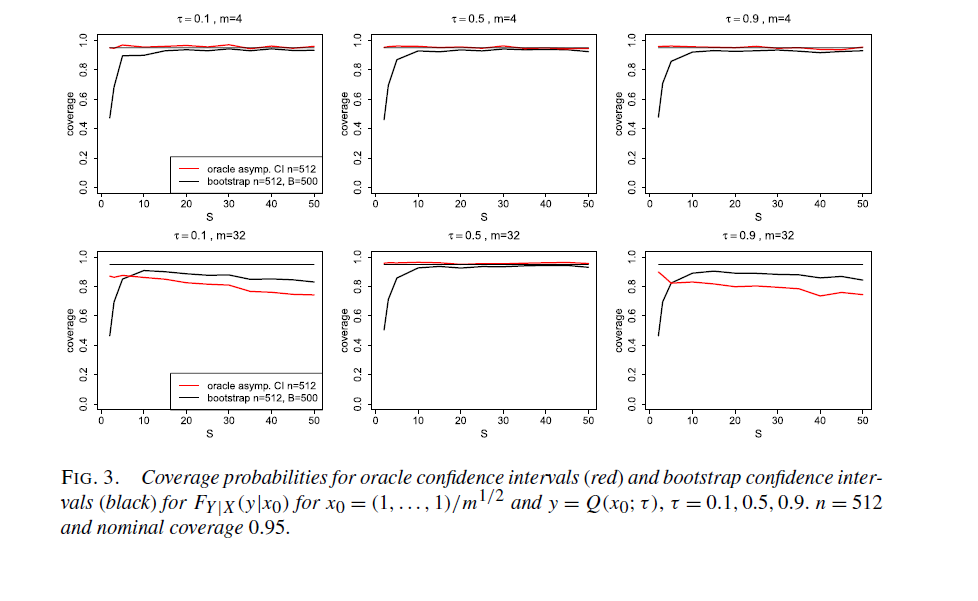
\includegraphics[scale=1]{fig3.png}
\end{frame}
\end{document}